% =====================================================================
%  Netzwerksicherheit - Praktische Aufgabe
%  Teilaufgaben: a) Wireshark/Telnet  b) nmap  c) macchanger
%                d) OWASP ZAP         e) Google Hacking
%
%  Kompilieren:  latexmk -pdf netzwerksicherheit_praxis.tex
%  (oder zweimal pdflatex laufen lassen, damit Referenzen/TOC stimmen)
% =====================================================================
\documentclass[11pt,a4paper]{article}

% ---------- Sprache & Encoding ----------
\usepackage[utf8]{inputenc}      % UTF-8 Quelltext (bei modernem TeX oft schon Default)
\usepackage[T1]{fontenc}         % korrekte Umlaut-Trennung & Glyphen
\usepackage[ngerman]{babel}      % deutsche Silbentrennung + "Abbildung"/"Tabelle"

% ---------- Layout ----------
\usepackage[a4paper,margin=2.5cm]{geometry}
\usepackage{parskip}             % Absatzabstand statt Einzug (Geschmackssache)

% ---------- Grafik & Floats ----------
\usepackage{graphicx}            % \includegraphics
\usepackage{float}               % ermoeglicht [H] = "genau hier" fuer Screenshots
\usepackage{caption}
\captionsetup{font=small,labelfont=bf}

% ---------- Code / Befehle / Ausgaben ----------
\usepackage{listings}
\usepackage{xcolor}

% Ein schlichter Stil fuer Terminal-/Code-Listings:
\definecolor{codebg}{rgb}{0.96,0.96,0.96}
\definecolor{codecomment}{rgb}{0.40,0.45,0.40}
\definecolor{codekw}{rgb}{0.10,0.20,0.55}

\lstdefinestyle{terminal}{
  backgroundcolor=\color{codebg},
  basicstyle=\ttfamily\small,
  commentstyle=\color{codecomment},
  keywordstyle=\color{codekw}\bfseries,
  breaklines=true,                 % lange Zeilen umbrechen
  breakatwhitespace=false,
  showstringspaces=false,
  frame=single,
  rulecolor=\color{black!20},
  numbers=none,
  tabsize=2,
  captionpos=b,
  literate=                        % Umlaute in Listings korrekt darstellen
    {ä}{{\"a}}1 {ö}{{\"o}}1 {ü}{{\"u}}1
    {Ä}{{\"A}}1 {Ö}{{\"O}}1 {Ü}{{\"U}}1 {ß}{{\ss}}1
}
\lstset{style=terminal}

% ---------- Links ----------
\usepackage{hyperref}
\hypersetup{
  colorlinks=true,
  linkcolor=black,                 % interne Verweise dezent
  urlcolor=blue!60!black,
  citecolor=black,
  pdftitle={Netzwerksicherheit - Praktische Aufgabe},
  pdfauthor={Martin Klejewski}
}

% =====================================================================
%  Titel
% =====================================================================
\title{Netzwerksicherheit\\\large Praktische Aufgabe: Wireshark, nmap, macchanger, OWASP ZAP, Google Hacking}
\author{Martin Klejewski}
\date{\today}

\begin{document}

\maketitle
\tableofcontents
\newpage

% =====================================================================
%  a) Wireshark / Telnet
% =====================================================================
\section{Wireshark: Telnet-Passwort aus \texttt{telnet.pcapng}}

% --- Hier kommt deine Erklaerung hin: Warum Telnet im Klartext uebertraegt,
%     welchen Weg du gewaehlt hast (Follow TCP Stream / Paket-fuer-Paket) ---

Telnet überträgt sämtliche Daten unverschlüsselt im Klartext, einschließlich
Benutzername und Passwort.
Um das Passwort zu finden, waren folgende Schritte notwendig:
\begin{enumerate}
	\item Die Datei \texttt{telnet.pcapng} wurde mit Wireshark geöffnet.
	\item Paket 11 ist das erste von Wireshark als Telnet erkannte Paket (die TCP-Verbindung selbst beginnt bei Paket 8).
	\item Der TCP Stream wurde gefolgt, um die Daten im Klartext zu sehen.
	\item Rechtsklick auf Paket 11 > Follow > TCP Stream (Alternativ: \texttt{Ctrl+Alt+Shift+F} auf Paket 11)
	\item Das Passwort wurde im Klartext sichtbar gemacht. (Abb. \ref{fig:a-stream})
\end{enumerate}


\begin{figure}[H]
  \centering
  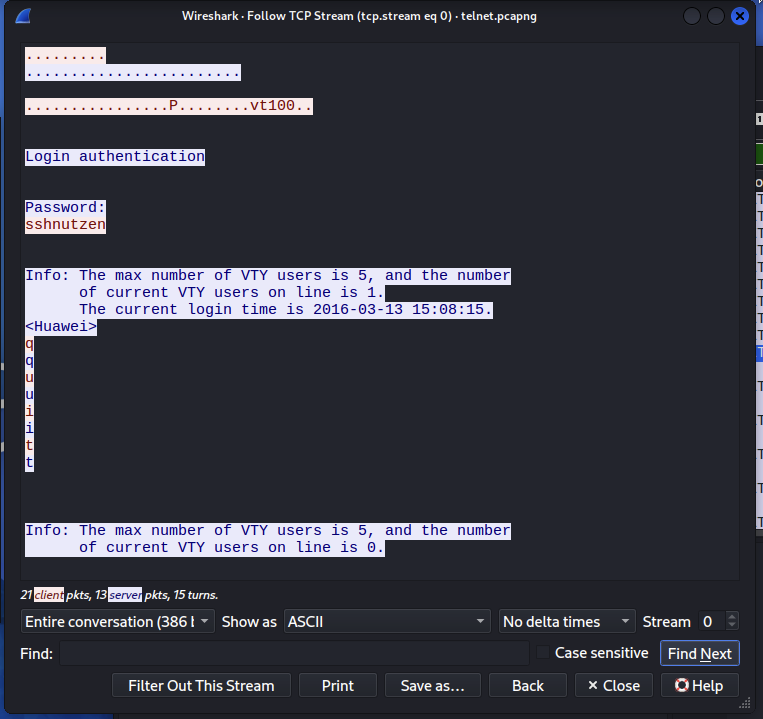
\includegraphics[width=\textwidth]{screenshots/screenshot_result_a.png}
  \caption{Follow TCP Stream: Benutzername und Passwort im Klartext sichtbar.}
  \label{fig:a-stream}
\end{figure}

\textbf{Ergebnis:} Gefundenes Passwort: \texttt{sshnutzen}.

% =====================================================================
%  b) nmap
% =====================================================================
\section{nmap: Scans des Testservers \texttt{nwsmooc.mooin.org}}

% --- Mindestens DREI Scans mit jeweils unterschiedlichen Parametern.
%     Jeweils: Befehl + Ausgabe + Erklaerung. ---

\subsection{Scan 1: \emph{(z.\,B. SYN-Scan / Top-Ports)}}

\begin{lstlisting}[caption={nmap-Befehl Scan 1}]
nmap -sS nwsmooc.mooin.org
\end{lstlisting}

\emph{Erklärung der Parameter und der Ausgabe hier.}

\begin{figure}[H]
  \centering
  % \includegraphics[width=0.9\textwidth]{screenshots/b_scan1.png}
  \caption{Ergebnis Scan 1.}
  \label{fig:b-scan1}
\end{figure}

\subsection{Scan 2: \emph{(z.\,B. Dienst-/Versionserkennung)}}

\begin{lstlisting}[caption={nmap-Befehl Scan 2}]
nmap -sV nwsmooc.mooin.org
\end{lstlisting}

\emph{Erklärung hier.}

\subsection{Scan 3: \emph{(z.\,B. Betriebssystemerkennung)}}

\begin{lstlisting}[caption={nmap-Befehl Scan 3}]
nmap -O nwsmooc.mooin.org
\end{lstlisting}

\emph{Erklärung hier.}

\subsection{Beobachtung in Wireshark}

\begin{figure}[H]
  \centering
  % 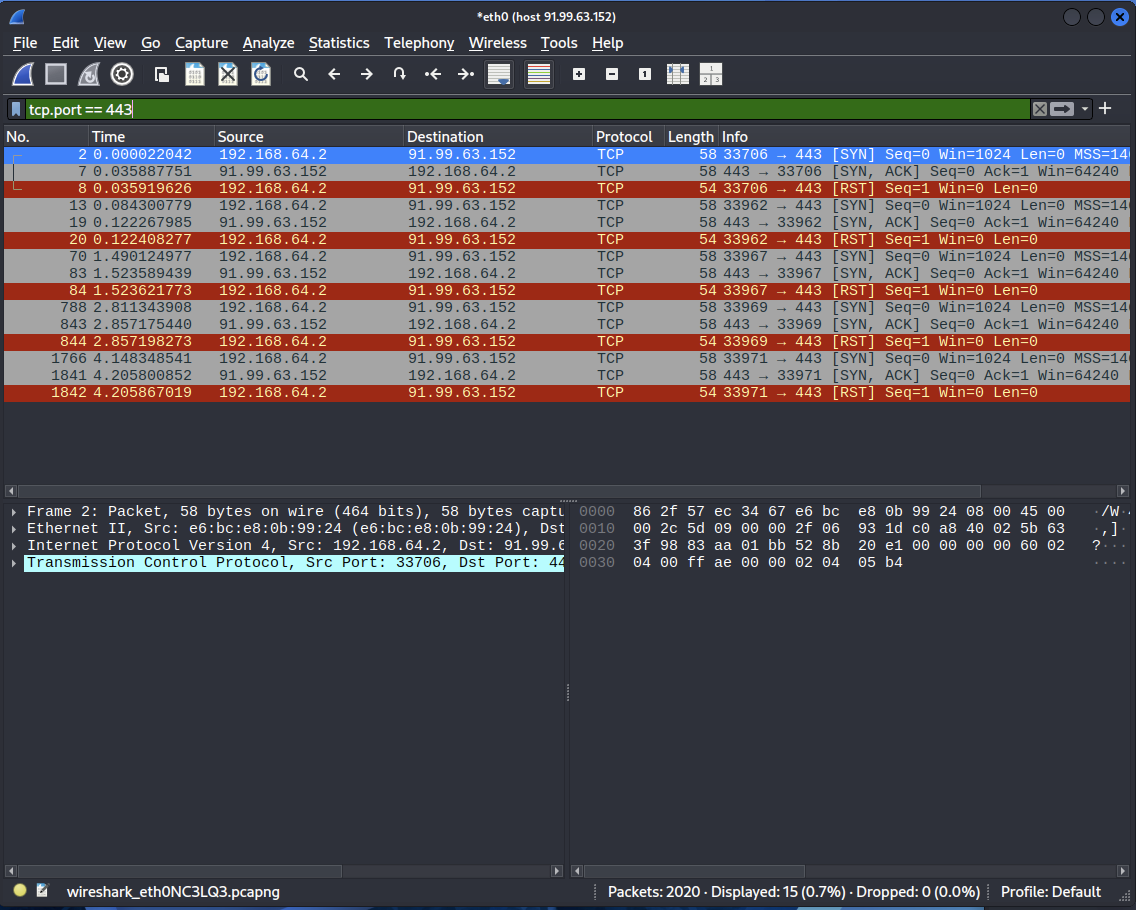
\includegraphics[width=0.9\textwidth]{screenshots/b_wireshark.png}
  \caption{Kommentierter Wireshark-Mitschnitt eines nmap-Scans.}
  \label{fig:b-wireshark}
\end{figure}

% =====================================================================
%  c) macchanger
% =====================================================================
\section{macchanger: Senden mit gefälschter MAC-Adresse}

% --- Was macchanger kann; Vorher/Nachher der MAC; wo die gefaelschte
%     Adresse in Wireshark sichtbar ist; wie es "richtig" waere. ---

\begin{lstlisting}[caption={Aktuelle MAC anzeigen und ändern}]
ifconfig
macchanger -r eth0
\end{lstlisting}

\emph{Erklärung hier: Was passiert, wie sähe der korrekte (echte) Wert aus,
wo ist die gefälschte MAC im Mitschnitt zu sehen?}

\begin{figure}[H]
  \centering
  % \includegraphics[width=0.9\textwidth]{screenshots/c_mac_wireshark.png}
  \caption{Gefälschte MAC-Adresse im Wireshark-Mitschnitt.}
  \label{fig:c-mac}
\end{figure}

% Optionaler zweiter Schritt: zusaetzlich IP-Adresse per DHCP neu anfordern.
% \subsection{Optional: Neuzuweisung der IPv4-Adresse}

% =====================================================================
%  d) OWASP ZAP
% =====================================================================
\section{OWASP ZAP: Schwachstellenanalyse von \texttt{https://nwsmooc.mooin.org}}

% --- Aktiver Scan (damit auch SQL Injection geprueft wird).
%     Die DREI relevantesten Findings auswaehlen und Kritikalitaet bewerten. ---

\emph{Kurzbeschreibung des Vorgehens (aktiver Scan aktiviert) hier.}

\subsection{Finding 1}
\emph{Beschreibung, Risiko/Kritikalität, mögliche Gegenmaßnahme.}

\begin{figure}[H]
  \centering
  % \includegraphics[width=0.9\textwidth]{screenshots/d_finding1.png}
  \caption{ZAP-Finding 1.}
  \label{fig:d-f1}
\end{figure}

\subsection{Finding 2}
\emph{Beschreibung und Bewertung.}

\subsection{Finding 3}
\emph{Beschreibung und Bewertung.}

% =====================================================================
%  e) Google Hacking
% =====================================================================
\section{Google Hacking: Drei Beispiele aus der GHDB}

% --- Drei selbstgewaehlte Dorks von exploit-db.com/google-hacking-database/
%     jeweils: Dork + was man damit findet + warum das ein Risiko ist. ---

\subsection{Beispiel 1}
\begin{lstlisting}[caption={Google-Dork Beispiel 1}]
<dork hier>
\end{lstlisting}
\emph{Was findet man damit, und warum ist das relevant?}

\subsection{Beispiel 2}
\begin{lstlisting}[caption={Google-Dork Beispiel 2}]
<dork hier>
\end{lstlisting}
\emph{Erklärung hier.}

\subsection{Beispiel 3}
\begin{lstlisting}[caption={Google-Dork Beispiel 3}]
<dork hier>
\end{lstlisting}
\emph{Erklärung hier.}

\end{document}
